\documentclass[11pt]{article}
\usepackage[margin=1in]{geometry}
\usepackage[T1]{fontenc}
\usepackage{lmodern}
\usepackage{microtype}
\usepackage{amsmath,amssymb,amsfonts}
\usepackage{booktabs}
\usepackage{array}
\usepackage{enumitem}
\usepackage{graphicx}
\usepackage{placeins}
\usepackage{xcolor}
\usepackage{hyperref}
\usepackage[numbers,sort&compress]{natbib}

\hypersetup{
  colorlinks=true,
  linkcolor=blue!55!black,
  citecolor=blue!55!black,
  urlcolor=blue!55!black
}

\setlist[itemize]{leftmargin=1.6em}
\setlist[enumerate]{leftmargin=1.8em}
\newcommand{\code}[1]{\texttt{#1}}
\newcommand{\R}{\mathbb{R}}
\newcommand{\E}{\mathcal{E}}
\newcommand{\tr}{\operatorname{tr}}
\newcommand{\diag}{\operatorname{diag}}
\newcommand{\vol}{\operatorname{vol}}
\newcommand{\argmin}{\operatorname*{arg\,min}}

\newenvironment{reviewbox}[1]
{\par\medskip\noindent\textbf{#1.}\ }
{\par\medskip}

\newcommand{\paperfigure}[4]{%
\begin{figure}[htbp]
\centering
\includegraphics[width=0.82\linewidth]{#1}
\caption{#2 Reproduced from #3, internal review only. #4}
\end{figure}
}


\title{Paper Review: Variable Bandwidth Diffusion Kernels}
\author{Writer-P04 polished review}
\date{Built 2026-05-15}

\begin{document}
\maketitle

\begin{abstract}
Berry and Harlim's \emph{Variable Bandwidth Diffusion Kernels}
\citep{berry2016variable} gives a precise answer to a question that appears
whenever graph weights are adapted to local sampling density: what continuum
operator is actually being approximated?  The paper shows that replacing a
global kernel scale by a local bandwidth \(\rho(x)\rho(y)\) is not a benign
implementation detail.  It changes both the finite-sample error and the
limiting differential operator unless it is paired with the right density
normalization.  Its central construction, especially the specialization
\(\rho=q^\beta\), is directly relevant to conductance-style comparisons for
SIMODS and \code{gflow}, but only as a proposed variable-bandwidth
Gaussian/RBF comparator.  It should not be retrofitted onto the current
overlap-density smoother without also adopting the paper's density estimate,
\(\alpha\)-normalization, row normalization, and final \(\rho^{-2}\) generator
scaling.
\end{abstract}

\section{Why This Paper Matters}

The usual fixed-bandwidth graph kernel treats a Euclidean distance the same
way everywhere in the data set.  Berry and Harlim study what happens when the
kernel scale is allowed to vary with position.  This is the mathematical
version of a familiar local-scale intuition: in a sparse tail, a point may need
to reach farther to find meaningful neighbors, while in a dense region the same
physical distance may already be too coarse.

The paper matters for a conductance and kernel-Laplacian review because it
separates three ideas that are often blurred together.  First, there is the raw
edge affinity.  Second, there is the density correction used before row
normalization.  Third, there is the differential operator obtained after the
kernel matrix is turned into a generator.  P04 shows that all three choices
affect the answer.  A local bandwidth can improve sparse-density behavior, but
it also introduces a drift term unless \(\alpha\), \(\beta\), and the intrinsic
dimension \(d\) are chosen to target a particular operator.

The paper's sign convention deserves an early warning.  Berry and Harlim use
\(\Delta\) for the negative of the usual Laplace--Beltrami operator and later
describe it as having negative eigenvalues.  The formulas below follow the
paper's convention.  When translating to SIMODS or graph-smoothing language,
one should check whether the implementation uses a generator convention,
a positive semidefinite graph Laplacian convention, or a conductance-energy
convention.

\section{Problem Setting and Reader Orientation}

The data are sampled from a density \(q\) on a \(d\)-dimensional Riemannian
manifold \(M\subset \R^n\).  Here \(d\) is the intrinsic dimension.  It is not
the ambient dimension, and it is not automatically the dimension of whatever
graph has been built from the data.  This point matters because \(d\) enters
the density estimate, the operator coefficients, and the error powers.

For fixed bandwidth, diffusion maps use kernels of the form
\[
  K_\epsilon(x,y)=h\!\left(\frac{\|x-y\|^2}{\epsilon}\right),
\]
and approximate, under the paper's sign convention, the operator
\[
  L_\alpha f
  = \Delta f + (2-2\alpha)\nabla f\cdot\frac{\nabla q}{q}.
\]
The parameter \(\alpha\) is the familiar Coifman--Lafon density
normalization \citep{coifman2006diffusion}.  At \(\alpha=1\), the sampling
density drift is removed and the limiting operator is the Laplacian.  At other
values, the density remains part of the diffusion geometry.

P04 asks for the corresponding theory when the bandwidth is local:
\[
  K_\epsilon^S(x,y)
  =
  h\!\left(\frac{\|x-y\|^2}{\epsilon\rho(x)\rho(y)}\right).
\]
The superscript \(S\) indicates the symmetric use of \(\rho\) at both endpoints.
The paper is partly motivated by self-tuned spectral clustering
\citep{zelnikmanor2004selftuning}, but its main contribution is not a new
clustering heuristic.  It is an asymptotic and finite-sample analysis of the
operator induced by these locally scaled kernels.

\section{Main Construction}

The practical Gaussian implementation in Section 3 is the most portable form
for a graph comparator:
\[
  K_\epsilon^S(x_i,x_j)
  =
  \exp\!\left(
    -\frac{\|x_i-x_j\|^2}{4\epsilon\rho(x_i)\rho(x_j)}
  \right).
\]
If \(x_i\) and \(x_j\) are close enough that
\(\rho(x_i)\approx\rho(x_j)\), the local length scale is approximately
\(2\sqrt{\epsilon}\rho(x_i)\).  Thus a negative density exponent, such as
\(\rho=q^{-1/2}\), enlarges the effective neighborhood in sparse regions and
shrinks it in dense regions.  This is a useful conductance analogy, but it is
only the first layer of the method.

\begin{figure}[htbp]
\centering
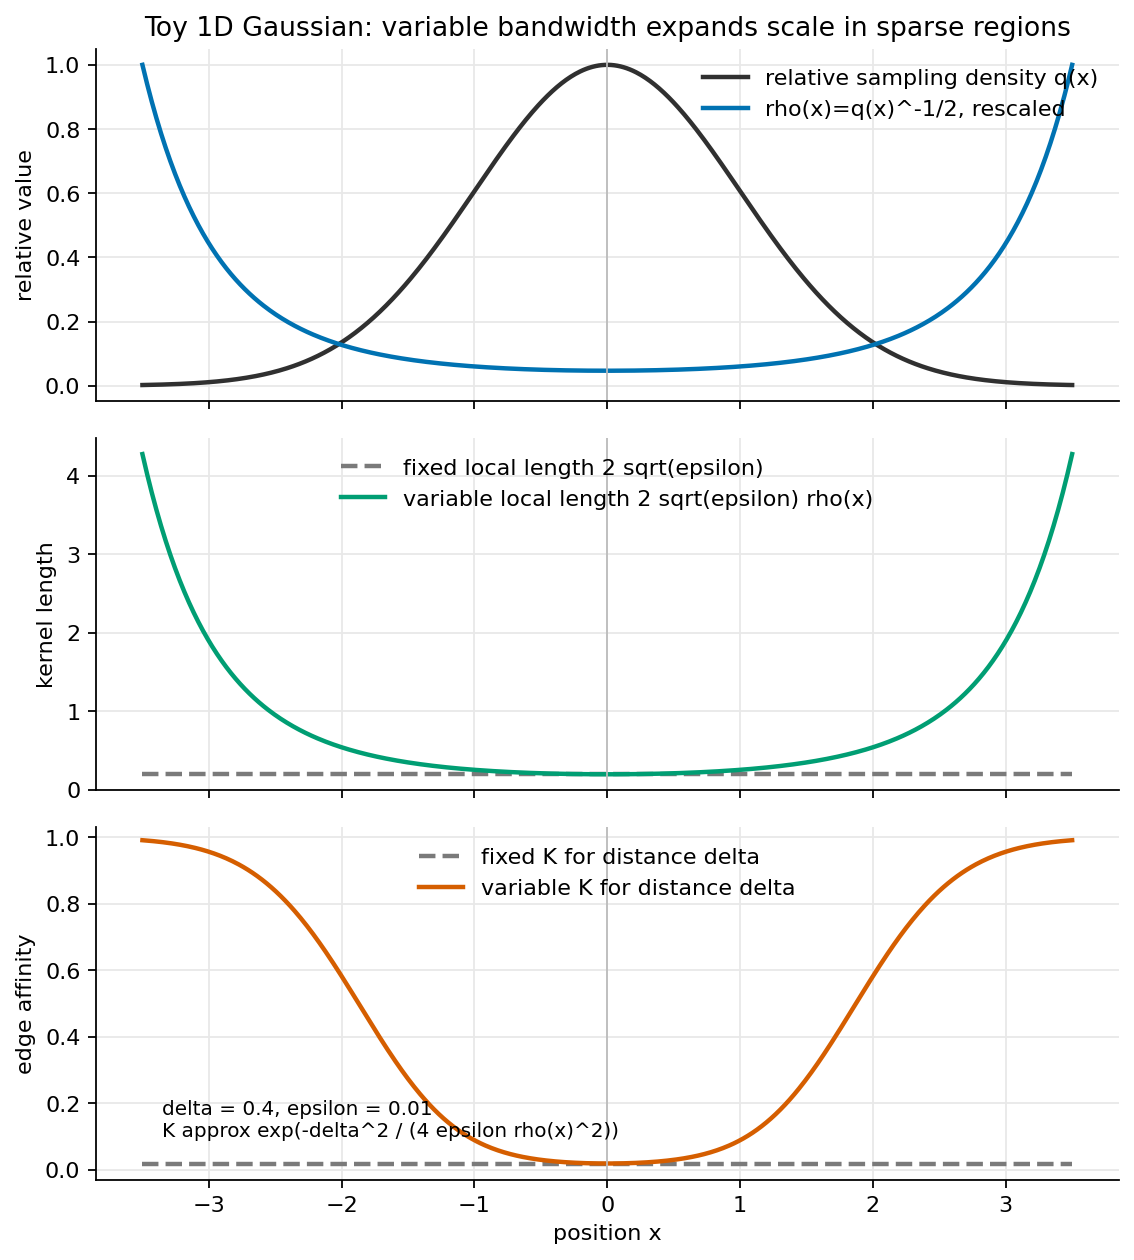
\includegraphics[width=0.78\linewidth]{../../figures/P04_local_bandwidth_conductance_curve.png}
\caption{Original explanatory figure for internal review.  For the Gaussian
implementation in P04, choosing \(\rho=q^{-1/2}\) makes the same physical
separation receive a larger affinity in sparse regions than in dense regions.
This figure is derived from the paper's kernel formula; it is not reproduced
from Berry and Harlim.}
\end{figure}

The second layer is the density correction.  Berry and Harlim estimate the
sampling density using the variable-bandwidth kernel itself,
\[
  q_\epsilon^S(x_i)
  =
  \frac{\sum_l K_\epsilon^S(x_i,x_l)}{\rho(x_i)^d}.
\]
The division by \(\rho(x_i)^d\) is not cosmetic.  The leading term of the
variable-bandwidth kernel density expansion is proportional to \(\rho^d q\);
dividing by \(\rho^d\) is what recovers \(q\) rather than a bandwidth-weighted
density.

The normalized kernel is then divided by
\((q_\epsilon^S(x_i)q_\epsilon^S(x_j))^\alpha\), row-normalized, and converted
to a generator by
\[
  L_{\epsilon,\alpha,\beta}^S(x_i,x_j)
  =
  \frac{\widehat K_{\epsilon,\alpha}^S(x_i,x_j)-\delta_{ij}}
       {\epsilon\rho(x_i)^2}.
\]
This last \(\rho(x_i)^{-2}\) factor is another place where the construction
departs from a plain symmetric graph Laplacian.  The operator used for
eigensolvers is a symmetric conjugate of this row-normalized generator, not the
unnormalized kernel matrix itself.

\section{Limiting Operators and Sparse-Density Error}

Theorem 1 states that, for smooth functions and under the paper's regularity
conditions, the discrete variable-bandwidth operator converges pointwise with
high probability to
\[
  L_{\alpha,\rho} f
  =
  \Delta f
  + 2(1-\alpha)\nabla f\cdot\frac{\nabla q}{q}
  + (d+2)\nabla f\cdot\frac{\nabla\rho}{\rho}.
\]
The extra \((d+2)\nabla\rho/\rho\) drift is the paper's key warning.  Local
bandwidth changes the continuum operator.  Even with uniform sampling, a
nonconstant \(\rho\) does not recover the Laplacian unless the construction is
chosen to cancel the induced drift.

The most important specialization is
\[
  \rho=q^\beta+O(\epsilon).
\]
Then the limiting operator becomes
\[
  L_{\alpha,\beta}f
  =
  \Delta f
  +
  c_1\nabla f\cdot\frac{\nabla q}{q},
  \qquad
  c_1 = 2-2\alpha+d\beta+2\beta.
\]
This formula makes \(\alpha\) and \(\beta\) operator-design parameters.  With
\(\beta=-1/2\), the paper uses \(\alpha=-d/4\) for a gradient-flow generator
with \(c_1=1\), and \(\alpha=1/2-d/4\) for a Laplacian target with \(c_1=0\).
The familiar fixed-bandwidth Laplacian case, \(\beta=0\), recovers the
Coifman--Lafon choice \(\alpha=1\).

The finite-sample result is equally important.  The high-probability error has
three parts: an \(O(\epsilon)\) continuum bias, a density-renormalization
sampling error, and a ratio-estimator sampling error.  Under
\(\rho=q^\beta\), the latter two contain powers of \(q(x_i)\).  The paper
summarizes the sparse-density condition by requiring
\[
  \frac{1-d\beta}{2}>0,
  \qquad
  c_2 < 0,
  \qquad
  c_2=\frac12-2\alpha+2d\alpha+\frac{d\beta}{2}+\beta.
\]
For fixed bandwidth with \(\beta=0\) and \(\alpha>0\), \(c_2\) is positive in
the usual settings, so the pointwise error can blow up where \(q\) is small.
This is the technical basis for the paper's claim that variable bandwidth is
not merely a nicer density estimator: for operator approximation on supports
where the density is not bounded away from zero, it can be necessary for
convergence.

\section{Figures, Experiments, and Evidence}

The experiments support the theorem's sparse-tail story.  On the real-line
Ornstein--Uhlenbeck example, fixed bandwidth can appear acceptable for a
carefully chosen small deterministic sample, but it becomes unstable as more
tail points enter the data.  Variable bandwidth keeps the fourth eigenfunction
close to the analytic curve across a much wider range of \(\epsilon\).

\paperfigure{../../paper_figures/P04_F01_F02_page07.png}
{Figures 1 and 2 show the practical consequence of the error powers in
Corollary 1: fixed bandwidth is highly sensitive to \(\epsilon\) and fails in
the tails, while the \(\beta=-1/2\) variable-bandwidth construction stays close
to the Ornstein--Uhlenbeck eigenfunction over a broad range.}
{Berry and Harlim (2016), PDF p. 7.}
{The screenshot is useful here because it shows both the eigenfunction
distortion and the wide low-error region for the variable-bandwidth kernel.}

The two-dimensional Ornstein--Uhlenbeck experiment repeats the same message on
\(\R^2\): the variable-bandwidth estimate of the analytic eigenfunction
\(\phi_4(x,y)=xy\) is visually reasonable, while the fixed-bandwidth estimate
is not, even after empirical tuning.  The compact-manifold experiments are more
subtle.  On the nonuniformly sampled circle and sphere, fixed bandwidth can
work if \(\epsilon\) is well chosen, but the variable-bandwidth kernel is less
sensitive and better aligned with the automatic \(\epsilon\)-tuning heuristic.

\paperfigure{../../paper_figures/P04_F06_page11.png}
{Figure 6 shows the compact-manifold case on a nonuniformly sampled circle.  The
variable-bandwidth kernel has a wider low-error range for the second Laplacian
eigenfunction, and the automatic tuning slope peaks near \(d/2=1/2\).}
{Berry and Harlim (2016), PDF p. 11.}
{For SIMODS, this figure is a reminder that local scale can reduce nuisance
bandwidth sensitivity even when the density is bounded away from zero.}

The appendix figures are not just checks of code; they verify the operator
identities that control interpretation.  Figure A.8 distinguishes left, right,
and symmetric bandwidth placements.  Figure A.9 verifies that with
\(\rho=q^\beta\), changing \(\alpha\) switches between a Laplacian target and a
backward Kolmogorov target.

\paperfigure{../../paper_figures/P04_FA9_page23.png}
{Figure A.9 verifies the \(\rho=q^\beta\) expansion on the circle.  With
\(\beta=-1/2\), the paper shows \(\alpha=1/4\) recovering the Laplacian case
and \(\alpha=-1/4\) recovering the drifted backward Kolmogorov case.}
{Berry and Harlim (2016), PDF p. 23.}
{This is the cleanest figure-level evidence that the same local bandwidth can
support different continuum operators depending on normalization.}

\section{Limitations and Transfer Risks}

The theorem proves pointwise convergence for smooth functions.  The numerical
sections compare eigenvectors with analytic eigenfunctions, and the evidence is
convincing as a demonstration, but the paper explicitly does not prove spectral
convergence for variable-bandwidth kernels.  It also excludes manifolds with
boundary, especially non-compact manifolds with non-compact boundary.  These
are not small technicalities for applications where the sampled support has
hard truncation, censoring, or project-specific boundary artifacts.

The requirement to know or estimate \(d\) is the main practical burden.  The
dimension is needed in the \(\rho^d\) density correction and in the coefficients
\(c_1\) and \(c_2\).  P04 suggests that the slope of an automatic
\(\epsilon\)-tuning statistic may provide a dimension estimate, but it does not
turn this into a robust dimension-estimation method.

A second transfer risk is terminological.  The paper defines kernel affinities
and row-normalized diffusion generators.  It does not define conductance in the
SIMODS or \code{gflow} sense.  The raw Gaussian weight
\[
  w_{ij}=
  \exp\!\left(
    -\frac{d_{ij}^2}{4\epsilon\rho_i\rho_j}
  \right)
\]
is a natural conductance-like edge-weight candidate for a future comparator,
but the paper's claims about Laplacian recovery, gradient-flow generators, and
sparse-density robustness apply to the full normalized operator, not to that
raw affinity alone.

\section{Implications for SIMODS and \code{gflow}}

For SIMODS, P04 is best read as a design specification for a possible
density-adaptive Gaussian comparator.  It supports the idea that local scale is
an operator parameter, not just a graph-construction convenience.  A comparator
could choose \(\rho_i\) from a pilot density estimate or a nearest-neighbor
scale, set \(w_{ij}\) by the variable-bandwidth Gaussian formula, and then
evaluate whether the intended smoothing target is Laplacian-like
(\(c_1=0\)) or density-biased/gradient-flow-like (\(c_1>0\)).

This should remain distinct from the current \code{fit.rdgraph.regression()}
semantics.  In the current project language, supplied \code{weight.list} values
are positive graph edge lengths used for local ordering and truncation, while
the current smoothing conductance is based on overlap-density/Riemannian-complex
structure, approximately \(c_e^\rho=1/\max(\rho_1(e),10^{-10})\) in the current
default regime.  That is separate from direct inverse-length conductance and
separate again from P04's Gaussian/RBF variable-bandwidth affinity.

The strongest project-level lesson is cautionary.  If a SIMODS experiment
borrows only the raw local-scale Gaussian weight, it should be described as a
kernel-conductance comparator inspired by P04.  If it claims a Berry--Harlim
operator limit, it must also specify \(q_\epsilon^S\), \(\alpha\), \(\beta\),
\(d\), row normalization, and the \(\rho^{-2}\) generator scaling.  Without
those ingredients, the continuum interpretation changes.

\section{What To Reuse}

The reusable mathematical object is the normalized variable-bandwidth operator,
not just the slogan that sparse regions get wider neighborhoods.  For future
comparisons, P04 suggests the following disciplined split.

\begin{enumerate}
\item Use the raw Gaussian formula as a conductance-like edge weight when the
goal is to compare local-scale affinities.
\item Track the normalization separately, because changing \(\alpha\) and
\(\beta\) changes the limiting drift.
\item Report the intrinsic dimension assumption or estimator, since \(d\)
controls both density correction and operator targeting.
\item Interpret sparse-tail improvements as an operator-estimation claim only
when the full P04 construction is used.
\end{enumerate}

\section*{Provenance}

Primary source: local canonical PDF
\path{sources/pdf/P04_berry_harlim_variable_bandwidth_diffusion_kernels.pdf},
read in full, including theorem statements, implementation details, numerical
figures, conclusion, and appendices.  Archival scaffolding: local memo
\path{paper_memos/P04_berry_harlim_variable_bandwidth_diffusion_kernels.md}
and audit
\path{audits/P04_berry_harlim_variable_bandwidth_diffusion_kernels_audit.md}.
Figure screenshots are internal-review captures listed in
\path{paper_figure_screenshots.yml}; the local-bandwidth conductance curve is
an original explanatory figure derived from the Section 3 Gaussian formula.

\bibliographystyle{plainnat}
\bibliography{../../references}

\end{document}
